%! TeX root = main.tex

\documentclass{article}
\usepackage{amsmath}
\usepackage{amssymb}
\usepackage{microtype}
\usepackage{amsthm}
\usepackage{colortbl}
\usepackage[T1]{fontenc}
\usepackage[margin=0.5in]{geometry}
\usepackage{color}   %May be necessary if you want to color links
\usepackage[pdfencoding=auto, psdextra]{hyperref}
\usepackage{mathtools}
\usepackage{tikz}
\usetikzlibrary{automata, positioning, arrows, arrows.meta}

\hypersetup{
    colorlinks=true, %set true if you want colored links
    linktoc=all,     %set to all if you want both sections and subsections linked
    linkcolor=blue,  %choose some color if you want links to stand out
}

\newcommand\tab[1][1cm]{\hspace*{#1}}

\newtheorem{theorem}{Theorem}[subsection]
\newtheorem{corollary}{Corollary}[subsection]
\newtheorem{proposition}{Proposition}[subsection]
\newtheorem{lemma}{Lemma}[subsection]
\newtheorem*{remark}{Remark}

\theoremstyle{definition}

\newtheorem{example}{Example}[section]
\newtheorem{subexample}{Example}[subsection]
\newtheorem{definition}{Definition}[section]
\newtheorem{subdefinition}{Definition}[subsection]

\title{\vspace{-1in}CS3231 Theory of Computation notes}
\author{Aloysius}
\date{August 2025}
\setlength\parindent{0pt}
\begin{document}
\maketitle
\tableofcontents

\section{Preliminaries}
\begin{definition}[Alphabet]
	An alphabet is a \textbf{finite}, non-empty set of symbols, usually denoted by the symbol \( \Sigma  \). e.g. \( \{0,1\}, \{A,B, \ldots , Z\}, \{0, A, s\} \)
\end{definition}
\begin{definition}[String]
	A string is a finite sequence of symbols from an Alphabet, e.g. 001011, ABZSFAJF, 0AAAss. The empty string is denoted as \( \epsilon  \)
\end{definition}
\begin{definition}[Language]
	A Language is a set of Strings over an alphabet.
\end{definition}

\begin{definition}[Powers on an Alphabet]
	The nth power of an alphabet, \( \Sigma ^{n}  \), is the set of all strings of length n over the alphabet. Note that \( \Sigma ^{*}  \) represents all strings of finite length over the alphabet.
\end{definition}
\begin{definition}[Concatenation of Strings]
	String concatenation operator is \( \cdot \), but it can be dropped.
\end{definition}

\begin{definition}[Operators on Languages]
\end{definition}
\begin{enumerate}
	\item \( L_{1}\cdot L_{2} = L_{1}L_{2} = \{xy: x \in L_{1}, y \in L_{2}\} \)
	\item \( L^{*} = \{x_{1}x_{2}\ldots x_n: x_{1},x_{2},\ldots ,x_n \in L, n \in \mathbb{N}\} = \epsilon \cup L \cup LL \cup LLL \cup \ldots  \)
	\item \( L^{+} = \{x_{1}x_{2}\ldots x_n: x_{1},x_{2},\ldots ,x_n \in L, n\ge 1\} = L \cup LL \cup LLL \cup \ldots \)
\end{enumerate}

\section{DFA, NFA, Regular expressions}
\subsection{DFA}
A Deterministic Finite automata is defined by 5 things
\begin{enumerate}
	\item A finite set of states, denoted as \( Q \)
	\item A finite set of symbols from an alphabet \( \Sigma  \)
	\item A transition function, that takes a state from \( Q \) and a symbol from \( \Sigma  \), and returns a state from \( Q \), denoted as \( \delta  \)
	\item A starting state, \( q_{0} \)
	\item A set of final/accepting states, denoted as \( F \)
\end{enumerate}

For example, a DFA can be constructed to accept any string containing an odd number of bs
\begin{itemize}
	\item \( \delta(q_{0}, a) = q_{0} \)
	\item \( \delta (q_{0}, b) = q_{1} \)
	\item \( \delta (q_{1}, a) = q_{1} \)
	\item \( \delta (q_{1}, b) = q_{0} \)
\end{itemize}

\( \hat{\delta }  \) is a function that takes in an initial state and a string, and accepts it if the DFA accepts the string.
\begin{align*}
	 & \text{Base case: }                                      \\
	 & \hat{\delta }(q, \epsilon ) = q                         \\
	 & \text{Inductive case: }                                 \\
	 & \hat{\delta }(q, wa) = \delta (\hat{\delta }(q, w), a )
\end{align*}

\begin{definition}[Dead state]
	A dead state is a state from which a final state can not be reached.
\end{definition}
\begin{definition}[Unreachable state]
	An unreachable state is a state \( q \) for which \( \forall w \in \Sigma ^{*}, \hat{\delta }(q_{0}, w) \neq q   \)
\end{definition}

\subsection{NFA}
A Non Deterministic Finite Automata is almost like a DFA, except it's transition function maps to a subset of states in \( Q \).
In practice, this means a state in a NFA diagram can have multiple arrows with the same symbol attached to it. This allows for more compact diagrams.

\subsection{Equivalence of DFA and NFA}
Given any NFA, we can treat every possible subset of \( Q \) as a state in the DFA, such that \( Q_D = \{S| S \subset Q\} \). The set of final states is the set of subsets of \( Q \) where there is at least one final state,
\( F_D = \{S| S \subset Q \land S \cap  F \neq \emptyset \} \). We can then define a transition function for the DFA as:
\[
	\delta_D(S, a) = \cup_{q \in S} \delta_N(q, a)
	.\]

Since an NFA can handle multiple states at once, this definition of a transition function basically simulates an NFA by finding all the possible states the NFA can be in. This is known as the Powerset construction.

\begin{proof}[Powerset construction]
	Claim: For any string \( w \), \( \hat{\delta_D}(\{q_{0}\}, w) = \hat{\delta_N}(q_{0}, w)   \)
	\begin{align*}
		                              & \text{Base case:}                                                     \\
		                              & \delta_D(\{q_{0}\}, \epsilon ) = \{q_0\} = \delta_N(q_{0}, \epsilon ) \\
		                              & \text{Inductive case:}                                                \\
		\hat{\delta_D}(\{q_{0}\}, wa) & = \delta_D(\hat{\delta _D}(\{q_{0}\}, w), a )                         \\
		                              & = \delta_D(\hat{\delta _N}(q_{0}, w), a )                             \\
		                              & = \cup_{q \in \hat{\delta _N}(q_{0}, w) } \delta (q, a)               \\
		                              & = \hat{\delta _N}(q_{0}, wa)                                          \\
	\end{align*}
\end{proof}

Hence any NFA can be converted into a DFA, and it follows that an NFA can not be constructed to accept a Language that a DFA can not accept.

\subsection{\texorpdfstring{\( \epsilon  \)}{\textepsilon}-NFA}
An \( \epsilon  \)-NFA is a NFA with a transition function that accepts empty strings, essentially it allows some states to have optional transitions.

\begin{definition}[Empty closure]
	The empty closure of a state in an \( \epsilon  \)-NFA is the set of states reachable by taking any amount of \( \epsilon  \) transitions

	\begin{enumerate}
		\item \( q \in Eclose(q) \)
		\item \( p \in Eclose(q) \implies \forall k \in \delta(p, \epsilon ), k \in  Eclose(q) \)
		\item Iterate step 2 until not more \( \epsilon  \) transitions can be taken
	\end{enumerate}
\end{definition}

The \( \hat{\delta }  \) of a \( \epsilon  \)-NFA is defined as follows:
\begin{align*}
	 & \text{Base case:}                                                                          \\
	 & \hat{\delta }(q, \epsilon ) = Eclose(q)                                                    \\
	 & \text{Inductive case:}                                                                     \\
	 & \hat{\delta }(q, wa)                                                                       \\
	 & \text{First, find all the set of all possible ending states:}                              \\
	 & R = \cup_{p \in \hat{\delta }(q, w) } \delta(p, a)                                         \\
	 & \text{Then, the string transition function is just the empty closure of the ending states} \\
	 & \hat{\delta }(q, wa) = \cup_{p \in R} Eclose(p)
\end{align*}

Naturally, \( \epsilon  \)-NFAs are equivalent to NFAs, which mean they are equivalent to DFAs as well. To convert an \( \epsilon  \)-NFA to a NFA, \( \delta_N(q, a) = \cup_{p \in Eclose(q)} Eclose(\delta_\epsilon(p,a)) \).

\subsection{Regular expressions}
A regular expression is equivalent to a DFA, given an alphabet \( \Sigma \), \( L(r) \) gives the set of strings accepted by the regular expression.
The grammar for a regular expression is as follows:
\begin{enumerate}
	\item \( \epsilon  \), where \( L(\epsilon ) = \{\epsilon \} \)
	\item \( \emptyset \), where \( L(\emptyset) = \emptyset \)
	\item \( a \), where \( a \in \Sigma  \) and \( L(a) = \{a\} \)
	\item \( r_{1}+r_{2} \), given two regular expressions, their union is represented by \( + \). \( L(r_{1}+r_{2}) = L(r_{1})\cup L(r_{2}) \)
	\item \( r_{1} \cdot r_{2} \), given two regular expressions, their concatenation is represented by \( \cdot \). \( L(r_{1}\cdot r_{2}) = \{xy| x \in L(r_{1}), y \in L(r_{2})\} \)
	\item \( r^{*}  \), given a regular expression, its kleene star is represented by \( * \). \( L(r^{*} ) = \{x_{1}x_{2}\ldots x_k | \forall  1 \le i \le k, x_i \in L(r) \} \).
	      Note that \( k \) can be 0, so \( \emptyset \in  L(r^{*} ) \)
	\item \( (r) \), a regular expression wrapped around a paranthesis
\end{enumerate}
Note that the precedence rule is \( * > \cdot > + \)

\subsubsection{DFA to Regular Expression}
A DFA can be converted to a regular expression very easily.
Given the DFA \( A = (Q, \Sigma, \delta, q_{0}, F) \), and assume that \( Q = \{1,2,\ldots n\} \) and \( q_{0} = 1 \).
Let \( R^{k}_{i,j}  \) be the regular expression that accepts the set of strings that moves the DFA from the state \( i \) to the state \( j \),
only using intermediary states numbered \( \le k \).

Base case, \( k=0 \).
\[
	R^{0}_{i,j} = \begin{cases}
		\sum_{\delta(i, a_i) = j} a_i,            & \text{ if }i \neq j \\
		\epsilon + \sum_{\delta(i, a_i) = i} a_i, & \text{ if }i = j    \\
	\end{cases}
	.\]

Induction case
\[
	R^{k+1}_{i,j} = R^{k}_{i,j} + R^{k}_{i,k+1} (R^{k}_{k+1, k+1})^{*}R^{k}_{k+1,j}
	.\]

The construction is simple, you take the regular expression for \( R^{k}_{i,j} \), then union it with the regular expression that takes \( i \) to \( k+1 \) (\( R^{k}_{i, k+1}  \)),
concatenated with any number of useless transitions (\( (R^{k}_{k+1,k+1})^{*}   \)), concatenated with the regular expression that takes \( k+1 \) to \( j \) (\( R^{k}_{k+1,j}  \)).

Hence a regular expression equivalent to the DFA would be
\[
	\sum_{j \in F} R^{n}_{1,j}
	.\]


\subsubsection{Regular Expression to \texorpdfstring{\( \epsilon  \)}{\textepsilon}-NFA}
A regular expression can be converted to an \( \epsilon  \)-NFA by applying some simple recursive transformations, which leads to an \( \epsilon  \)-NFA with the following properties:
\begin{enumerate}
	\item It has only one final state
	\item There is no transition into the final state
	\item There is no transition out of the final state
	\item The starting and final states are different
\end{enumerate}
The transformation rules are as follows, note that if a state does not have a transition, it goes to a dead state.
\begin{enumerate}
	\item \( \emptyset \): \( A = (\{q_{0}, q_f\}, \Sigma , \delta , q_{0}, \{q_f\}) \), where \( q_{0} \) is a dead state.
	\item \( \epsilon  \): \( A = (\{q_{0}, q_f\}, \Sigma , \delta , q_{0}, \{q_f\}) \), where \( \delta(q_{0}, \epsilon ) = q_f \) is the only transition.
	\item \( a \): \( A = (\{q_{0}, q_f\}, \Sigma , \delta , q_{0}, \{q_f\}) \), where \( \delta (q_{0}, a) = q_f \) is the only transition.
	\item \( r_{1}+r_{2} \):
	      Let \( A_{1} = (Q_{1}, \Sigma, \delta_{1} , q_{0}^{1} , q_f^{1} ) \) and \( A_{2} = (Q_{2}, \Sigma, \delta_{2} , q_{0}^{2} , q_f^{2} ) \)
	      represent the \( \epsilon  \)-NFA for \( r_{1} \) and \( r_{2} \) respectively.
	      Our new \( \epsilon  \)-NFA combines these two, where \( A = (\{q_{0}, q_f\} \cup Q_{1} \cup Q_{2}, \Sigma, \delta , q_{0} , \{q_f\} ) \) and
	      \begin{itemize}
		      \item \( \delta (q_{0}, \epsilon ) = \{q_{0}^{1}, q_{0}^{2}  \} \)
		      \item \( \delta (q_f^{1}, \epsilon  ) = q_f \)
		      \item \( \delta (q_f^{2}, \epsilon  ) = q_f \)
	      \end{itemize}
	      Additionally, \( \delta  \) contains all the transitions of \( \delta_{1} \) and \( \delta_{2} \)
	\item \( r_{1}\cdot r_{2} \):
	      Let \( A_{1} = (Q_{1}, \Sigma, \delta_{1} , q_{0}^{1} , q_f^{1} ) \) and \( A_{2} = (Q_{2}, \Sigma, \delta_{2} , q_{0}^{2} , q_f^{2} ) \)
	      represent the \( \epsilon  \)-NFA for \( r_{1} \) and \( r_{2} \) respectively.
	      Our new \( \epsilon  \)-NFA combines these two, where \( A = (\{q_{0}, q_f\} \cup Q_{1} \cup Q_{2}, \Sigma, \delta , q_{0} , \{q_f\} ) \) and
	      \begin{itemize}
		      \item \( \delta (q_{0}, \epsilon ) = \{q_{0}^{1} \} \)
		      \item \( \delta (q_f^{1}, \epsilon  ) = \{q_{0}^{2} \} \)
		      \item \( \delta (q_f^{2}, \epsilon  ) = \{q_f\} \)
	      \end{itemize}
	      Additionally, \( \delta  \) contains all the transitions of \( \delta_{1} \) and \( \delta_{2} \)
	\item \( r^{*}  \):
	      Let \( A_{1} = (Q_{1}, \Sigma, \delta_{1} , q_{0}^{1} , q_f^{1} ) \) represent the \( \epsilon  \)-NFA for \( r \).
	      Our new \( \epsilon  \)-NFA applies the kleene star rule, where \( A = (\{q_{0}, q_f\} \cup Q_1, \Sigma, \delta , q_{0} , \{q_f\} ) \) and
	      \begin{itemize}
		      \item \( \delta (q_{0}, \epsilon ) = \{q_{0}^{1}, q_f \} \)
		      \item \( \delta (q_{f}, \epsilon ) = \{q_{0}^{1}, q_f \} \)
	      \end{itemize}
	      Additionally, \( \delta  \) contains all the transitions of \( \delta_{1} \)
\end{enumerate}

\subsection{Minimization of DFA}
\begin{definition}[\( \equiv_L \)]
	Given a language L, \( u \equiv_L w \iff \forall x \in \Sigma ^{*} , ux \in L \iff wx \in L \), meaning \( ux \in L \) and \( wx \in L \), or \( ux \not \in L \) and \( wx \not \in L \)
\end{definition}

\( \equiv_L \) forms an equivalent relation, meaning it is reflexive, symmetric, and transitive. Let \( equiv(w) \) denote the equivalence class of w formed from \( \equiv_L \).
If \( | \{equiv(w) | w \in \Sigma ^{*} \} | \) is finite, then it forms a DFA \( (Q, \Sigma , \delta , q_{0}, F) \) where
\begin{itemize}
	\item \( Q = \{equiv(w) | w \in \Sigma ^{*}  \} \)
	\item \( q_{0} = equiv(\epsilon ) \)
	\item \( F = \{equiv(x) | x \in L\} \)
	\item \( \delta (equiv(w), a) = equiv(wa) \)
\end{itemize}

In this DFA, we are basically grouping strings into different classes based on their behaviour, any two strings in the same class will lead to the same state given the same continuation.
The DFA formed is minimal, meaning there is no other DFA for L with a smaller number of states. We can prove this by showing that a DFA for L must have at least the number of equivalence classes under \( \equiv_L \).

Claim: Every DFA for L must have at least the number of equivalent classes formed under \( \equiv_L \). This is equivalent to the statement \( u \not\equiv_L w \implies \hat{\delta}(q_{0}, u) \neq \hat{\delta (q_{0}, w)}   \)
\begin{proof}
	Suppose otherwise, that \( u \not \equiv_L w \implies \hat{\delta }(q_{0}, u) = \hat{\delta }(q_{0}, w)   \).
	This means that there exists a smaller DFA that can place two strings into the same state even though they were from different classes.

	Then, by definition of \( \equiv_L \), there exists some string \( x \) such that \( ux \in L \) and \( wx \not \in L \) or vice versa.
	However, \( \hat{\delta (q_{0}, ux)} = \hat{\delta (q_{0}, wx)}   \), meaning \( ux \) and \( wx \) must either be both in L, or not, hence a contradiction.
\end{proof}

The intuition behind why this works is because we are finding the minimal number of classes of strings that behave differently, if two equivalent classes behaved the same way, they would not be separate.
For example, given \( \Sigma = \{a,b\} \) and \( L = \{w | w \text{ ends with } a\} \), we have two equivalent classes, the set of strings ending in \( a \) and the set of strings ending in \( b \).
\( a \not \equiv_L b  \) because \( a \cdot \epsilon \in L \) but \( b\cdot \epsilon \not \in L \), hence our DFA only needs two states as \( equiv(\epsilon ) = equiv(b) \).

\subsubsection{Minimization algorithm}
First we need to find all distinguishable pairs of states. We say that \( (p, q) \) is distinguishable iff there exists a w such that \[
	\hat{\delta }(p, w) \in F \iff \hat{\delta }(q, w) \in F
	.\]
\begin{enumerate}
	\item Initialise all pairs (p,q) where \( p \in F \) and \( q \not \in F \), where they are all distinguishable pairs
	\item For any \( a \in \Sigma  \), if \( \delta (p, a) \) and \( \delta (q, a) \) form a distinguisable pair, then \( p \) and \( q \) are distinguishable
	\item Continue step 2 until no more distinguishable pairs can be formed, then the remaining pairs are indistinguishable
\end{enumerate}

Once we have all the indistinguishable pairs, they form their own equivalence classes, if \( \delta (p, a) = q \),
then \( \delta (Ep, a) = Eq \), where \( Ep \) and \( Eq \) are the equivalence classes for \( p \) and \( q \).

Initial state is the equivalence class containing the start state, final states are all equivalence classes containing final states.

\subsection{Properties of Regular languages}
\begin{theorem}[Pumping lemma]
\end{theorem}
Let \( L \) be a regular language, then there exists a constant \( n \) for \( L \) such that for any string \( w \in L \) where \( |w| \ge n \), then we can break \( w \) into 3 strings \( w = xyz \) such that
\begin{enumerate}
	\item \( y \neq \epsilon  \)
	\item \( |xy| \le n \)
	\item For all \( k \ge 0 \), the string \( xy^{k}z \in L  \)
\end{enumerate}

\textbf{Proof: } Consider the DFA for a regular language L which has \( n \) states and a string \( w \) of length at least \( n \), let \( q_{0} \) be the initial state and \( q_{1},q_{2},\ldots q_n \)
be the subsequent states after accepting the next \( n \) characters of \( w \). Since the DFA only has \( n \) states but we have visited \( n+1 \) states, by pigeonhole principle there must be at least 1 state repeated.
Lets call this repeated state \( q_s \), let \( x \) be the substring that ends up in the first occurence of \( q_s \), let \( y \) be the next substring that ends up in the repeated occurence of \( q_s \).
Then let \( z \) be the rest of the string \( w \). Since \( q_s = \hat{\delta }(q_{0}, x) = \hat{\delta }(q_0, xy)  \), then \( \forall k \in \mathbb{N}, q_s = \hat{\delta}(q_0, xy^{k} )  \)

\subsubsection{Decision problems}
\begin{enumerate}
	\item To decide if L is the empty set, check if all the final states are unreachable
	\item To decide if L is \( \Sigma ^{*}  \), take the complement of the DFA and check if all the final states are unreachable
\end{enumerate}

\subsection{Parallel simulation of DFA}
Given two DFAs, \( A = (Q, \Sigma , \delta , q_{0}, F) \) and \( A^{\prime} = (Q^{\prime}, \Sigma , \delta ^{\prime}, q_{0}^{\prime}, F^{\prime}    )  \), we can do a parallel simulation to run both DFAs.

Construct another DFA \( A^{\prime\prime} = (Q \times Q^{\prime}, \Sigma , \delta ^{\prime\prime}, (q_{0}, q_{0}^{\prime}, F^{\prime\prime}  )  )  \),
where \( \delta ^{\prime\prime}((q, q^{\prime}), a ) = (\delta (q, a), \delta ^{\prime}(q^{\prime}, a ) )  \), and \( F^{\prime\prime}  \) depends on the need.

For example, if we are trying to find the intersection of two languages, then \( F^{\prime\prime} = \{(q, q^{\prime} ): q \in F \land q^{\prime} \in F  \}  \).
If we are trying to find the union of two languages, then \( F^{\prime\prime} = \{(q, q^{\prime} ): q \in F \lor q^{\prime} \in F  \}  \).

\subsection{Homomorphism}
Suppose \( \Sigma  \) and \( \Gamma  \) are two alphabets. Suppose h is a
mapping from \( \Sigma  \) to \( \Gamma ^{*}  \). Extend h to strings as follows.

\begin{math}
	h(\epsilon ) = \epsilon . \\
	h(aw) = h(a) \cdot h(w), \text{ for any } a \in  \Sigma , w \in \Sigma ^{*} .
\end{math}

Above h is called a homomorphism.
If L is regular then h(L) = \( \{h(w) | w\in L\} \) is also regular. Likewise if \( h(L) \) is irregular, then L is irregular.


\subsection{Summary of proven statements}
\begin{itemize}
	\item Number of strings over any fixed finite alphabet \( \Sigma  \) is countable
	\item Number of languages over any non-empty alphabet is uncountable
	\item DFA is equivalent to NFA is equivalent to \( \epsilon  \)-NFA is equivalent to RegLangs
	\item RegLang properties:
	      \begin{itemize}
		      \item M+N = N+M
		      \item L(M+N) = L(M) + L(N)
		      \item L + L = L
		      \item \( (L^{*})^{*}  = L^{*}   \)
		      \item \( \emptyset ^{*} = \epsilon   \)
		      \item \( \epsilon ^{*} = \epsilon   \)
		      \item \( L^{+} = LL^{*} = L^{*}L \)
		      \item \( L^{*} = \epsilon  + L^{+}  \)
		      \item \( (L + M )^{*}  = (L^{*} M ^{*} )^{*}  \)
	      \end{itemize}
	\item If a language has n equivalence classes, it must have at least n states
	\item Closure properties of RegLangs:
	      \begin{enumerate}
		      \item If \( L_{1} \) and \( L_{2} \) are regular, then so is \( L_{1} \cup L_{2} \)
		      \item If \( L_{1} \) and \( L_{2} \) are regular, then so is \( L_{1} \cdot L_{2} \)
		      \item If \( L_{1} \) and \( L_{2} \) are regular, then so is \( L_{1} \cap L_{2} \)
		      \item If \( L_{1} \) and \( L_{2} \) are regular, then so is \( L_{1} - L_{2} \)
		      \item If \( L_{1} \) and \( L_{2} \) are regular, then so is \( L_{1} \cdot \overline{L_{2}}  \)
		      \item If \( L \), is regular, then so is \( \overline{L}  \)
		      \item If \( L \), is regular, then so is \( L^{R}   \)
		      \item If \( L \), is regular, then so is \( h(L) \)
		      \item If \( h(L) \) is irregular, then L is irregular.
	      \end{enumerate}
\end{itemize}

\subsection{Languages known to be regular or irregular}
Regular:
\begin{itemize}
	\item Strings that contain odd number of bs over \( \{a, b\} \)
	\item strings that contain 00 as a substring
	\item \( L = \{w | \text{ n-th symbol in w from the end is 1} \}. \)
	\item An integer that is \(  (+, -, \epsilon ) \) followed by digits
	\item \( \{w | \text{ number of a’s in w is of form 3i + 1, for some natural number i} \} \) (Tutorial 1 Q4a)
	\item \( \{w | w \text{ has abaab as a substring}\} \) (Tutorial 1 Q4b)
	\item \( \{w | w \text{ does not contain ababba as a substring}\} \) (Tutorial 1 Q4c)
	\item (Odd number of a’s and no b’s) or (any number of a’s followed by a b followed by even number of a’s) (Tutorial 1 Q5)
	\item \( \{w | w = a_1 b_1 a_2 b_2 \ldots  a_n b_n , \text{ for some n, where } a_i , b_i \in  \{0, 1\} \text{ and } a_1 a_2 \ldots  a_n >  b_1 b_2 \ldots  b_n \} \)
	\item Set of strings that end in bba
	\item For a string x, let \( x_i \) denote the i-th character in x. That is, x = \( x_{1}x_{2}x_{3}\ldots x_n \),
	      where n is the length of x and each \( x_i \in \Sigma  \).
	      Suppose L is regular. Then \( \{x : \exists r \in N, |x| = 2r \land x_{1}x_{3}x_{5}\ldots x_{2r-1} \in L\} \) is also regular.
	\item \( \{wxw^{ R} | w, x \in  \{a, b\}^{+}  \} \)
	\item Half(L) is regular
\end{itemize}
Irregular:
\begin{itemize}
	\item \( \{a^mb^m | m \ge  1\} \)
	\item \( \{a^ib^j | i < j\} \)
	\item \( \{a^p | p is prime\} \)
	\item \( \{wcw^{R} | w \in \{a,b\}^{*}  \} \) (Tutorial 3 q3a)
	\item \( \{ww | w \in \{a, b\}^{*} \} \) (Tutorial 3 q3b)
	\item \( \{a^{m}  : m > 0 \text{ and binary representation of m has even number of bits}\} \)
\end{itemize}

\section{Context Free Grammars}
\subsection{CFG}
\subsubsection{Definition}
A CFG is a 4 tuple \( G = (V, T, P, S) \) where
\begin{itemize}
	\item \( V \) is a finite set of non terminals
	\item \( T \) is a finite set of terminals
	\item \( P \) is a finite set of production rules \( A \to \gamma  \) where \( A \in V \) and \( \gamma  \in (V U T)^{*}  \)
	\item \( S \) is the starting symbol, and \( S \in V \)
\end{itemize}

\subsubsection{Derivation}
\( \alpha A \beta \Rightarrow \alpha \gamma \beta \) if there exists a production rule of the form \( A \to \gamma  \).
\( \alpha  \Rightarrow_G^*  \beta \) if there is a series of zero or more production rules that derives beta from alpha.

If \( S \Rightarrow_G^* \alpha  \), then \( \alpha  \) is a sentential form. Basically any string of terminals and non terminals that can be reached from \( S \) is a sentential form.

\subsubsection{Parsing}
Using left most derivation, we apply the production rule on the left most non terminal. Likewise for right most derivation, we apply the production rule on the right most non terminal.

A parse tree is generated when generating a string of non terminals from the starting symbol \( S \). For example:

\begin{figure}[ht]
	\centering
	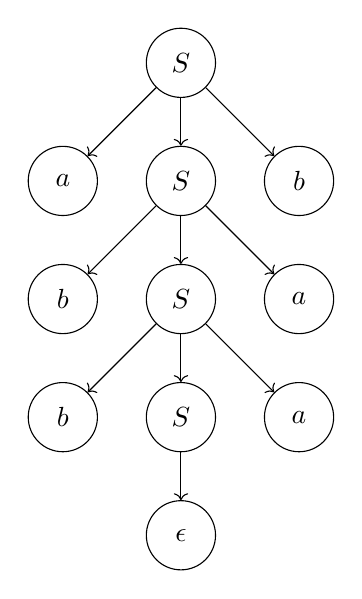
\begin{tikzpicture}
		\node[state] (S) {\( S \)};
		\node[state, below of=S, yshift=-0.5cm] (S1) {\( S \)};
		\node[state, below of=S, yshift=-0.5cm, xshift=-1.5cm] (a1) {\( a \)};
		\node[state, below of=S, yshift=-0.5cm, xshift=1.5cm] (b1) {\( b \)};
		\node[state, below of=S1, yshift=-0.5cm] (S2) {\( S \)};
		\node[state, below of=S1, yshift=-0.5cm, xshift=-1.5cm] (b2) {\( b \)};
		\node[state, below of=S1, yshift=-0.5cm, xshift=1.5cm] (a2) {\( a \)};
		\node[state, below of=S2, yshift=-0.5cm] (S3) {\( S \)};
		\node[state, below of=S2, yshift=-0.5cm, xshift=-1.5cm] (b3) {\( b \)};
		\node[state, below of=S2, yshift=-0.5cm, xshift=1.5cm] (a3) {\( a \)};
		\node[state, below of=S3, yshift=-0.5cm] (eps) {\( \epsilon  \)};

		\draw[->] (S) edge (b1);
		\draw[->] (S) edge (a1);
		\draw[->] (S) edge (S1);
		\draw[->] (S1) edge (b2);
		\draw[->] (S1) edge (a2);
		\draw[->] (S1) edge (S2);
		\draw[->] (S2) edge (b3);
		\draw[->] (S2) edge (a3);
		\draw[->] (S2) edge (S3);
		\draw[->] (S3) edge (eps);
	\end{tikzpicture}
\end{figure}

\subsubsection{Linear grammar}
A right linear grammar is a grammar where all production rules are of the form
\begin{align*}
	A \to wB, B \in V, w \in T^{*} \text{ or} \\
	A \to w, w \in T^{*}
\end{align*}

Likewise a left linear grammar is a grammar where all production rules are only to strings of terminals, or a non terminal followed by a string of terminals.

Linear grammars are equivalent to regular expressions.

\subsubsection{Ambiguous grammars}
A grammar is ambiguous if there exists two distinct parse trees to get to the same string of non terminals.
Some grammars can be disambiguated by changing the production rules, but some grammars are inherently ambiguous.

\subsection{PDA}
A push down automata is like a finite state machine but with a stack. More formally it is defined by the 7 tuple \( P = (Q, \Sigma , \Gamma , \delta , q_{0}, Z_{0}, F) \), where
\begin{itemize}
	\item \( Q, \Sigma ,q_{0}, F \) are like in a DFA
	\item \( \Gamma  \) is the stack alphabet
	\item \( Z_{0} \) is the only and initial symbol on the stack
	\item \( \delta  \) is a transition function from \( Q \times \Sigma \times \Gamma  \) to \( \mathcal{P}(  Q \times \Gamma ^{*})  \)
\end{itemize}

\( (p, \gamma ) \in \delta (q, a, X) \) indicates that at state \( q \), after reading input character \( a \),
and popping the top of the stack to get \( X \), the machine can travel to state \( p \), and push \( \gamma  \) onto the stack.
\( \gamma \in \Gamma ^{*}  \), and we push characters from right to left.
Note that we must always pop something from the top of the stack, we cannot progress if the stack is empty.

\subsubsection{Instantaneous description}
We say that \( (q, aw, X \alpha ) \vdash (p, w, \beta \alpha ) \) if \( (p, \beta ) \in \delta (q, aw, X) \)

\subsubsection{Language acceptance}
We can either accept by final state, if \[
	\{w | (q_{0}, w, Z_{0}) \vdash ^{*} (q_f, \epsilon , \alpha ) \text{ for some } q_f \in F  \}
	.\]

or by empty stack, if \[
	\{w | (q_{0}, w, F) \vdash ^{*} (q, \epsilon , \epsilon ) \text{ for some } q \in Q  \}
	.\]

Acceptance by final state or by empty stack is equivalent in a non deterministic PDA

\subsubsection{Deterministic PDA}
A deterministic PDA is just like a NPDA, but there is only one possible next move at each state, input character, and top of stack symbol.
So the transition function is from \( Q \times \Sigma \times \Gamma  \)  to \( Q \times \Gamma ^{*}  \).
And if there is an epsilon transition at state \( q \) and top of stack \( X \), then there can be no other transitions for any other input symbol \( a \in \Sigma  \).

A deterministic PDA is strictly weaker than a NPDA, and the language it accepts it forms the class of deterministic context free languages.
Acceptance by final state is also more powerful than acceptance by empty stack. Final state acceptance can accept all regular languages,
but empty stack can only accept a subset of final state, namely languages where for any \( x, y \in L \), \( x \) is not a prefix of \( y \).

\subsection{Procedures}
There are a few procedures that transforms grammars into simpler grammars but still express the same language

\subsubsection{Generating symbols}
A symbol \( A \) is generating if \( A \Rightarrow_G^* w \) for some \( w \in T ^{*}  \)

Non generating symbols in a grammar is useles, so lets get rid of them.
\begin{enumerate}
	\item Set all terminal symbols in the grammar to be generating
	\item If there exists a production of the form \( A \to w \), where every symbol in \( w \) is generating, then \( A \) is generating.
	\item Repeat step 2 until no more symbols can be added, then we can get rid of non generating symbols.
\end{enumerate}

\subsubsection{Reachable symbols}
A symbol \( A \) is reachable if \( S \Rightarrow_G^* \alpha A \beta  \), for some \( \alpha ,\beta  \in (V \cup T)^{*}  \)

Even if a symbol is generating, it may not be reachable from the starting symbol, such symbols are also useless, so lets get rid of them.
\begin{enumerate}
	\item \( S \) is reachable
	\item If \( A \to \alpha  \) and \( A \) is reachable, then all symbols in \( \alpha  \) are reachable.
	\item Repeat step 2 until no more symbols can be added, then we can get rid of non reachable symbols.
\end{enumerate}

\subsubsection{Useless symbols}
A symbol is useful only if it is reachable and generating. To get rid of useless symbols, first get rid of non generating symbols, then get rid of non reachable symbols.

\subsubsection{\texorpdfstring{\( \epsilon  \)}{\textepsilon} productions}
An \( \epsilon  \) production is a production rule that can lead to the empty string. We want to eliminate such productions

First we need to identify nullable symbol. A nullable symbol is one where \( A \Rightarrow_G^* \epsilon  \).
\begin{enumerate}
	\item For all \( A \to \epsilon  \), set \( A \) as nullable
	\item If \( A \to \alpha  \) and every symbol in \( \alpha  \) is nullable, then \( A \) is nullable
	\item Repeat step 2 until no more nullable symbols can be added
\end{enumerate}

Then to remove all \( \epsilon  \) productions, we do the following:
\begin{enumerate}
	\item First, designate all non terminals \( A \) where \( A \Rightarrow_G^* \epsilon  \) as nullable.
	\item Then, we want to remove all such productions that can lead to an empty string.
	      For each production \( B \to \alpha  \), where \( \alpha  \) contains one or more nullable non terminals,
	      replace it with all possible productions \( B \to \alpha ^{\prime}  \), which can be formed by removing some nullable non terminals in \( \alpha  \)
\end{enumerate}

If \( S \) is nullable, then the new language accepts the original language, except the empty string.

\subsubsection{Unit productions}
If \( A \Rightarrow_G^* B \), and \( B \in V \), then \( A \Rightarrow_G^* B \) is a unit production.

To get rid of such a unit production, we need to find all non unit productions \( B \to \gamma  \), and add \( A \to \gamma  \), and remove all productions of the form \( A \to C \) where \( C \in V \).

To do this, we need to find all unit pairs \( (A, B) \) where \( A \Rightarrow_G^* B \)
\begin{enumerate}
	\item \( \forall A \in V, (A,A) \) is a unit pair
	\item If \( (A, B) \) is a unit pair, and \( B \to C \), then \( (A, C) \) is a unit pair.
\end{enumerate}

All unit pairs are unit productions

\subsubsection{Chomsky normal form}
Every grammar can be converted to a chomsky normal form, where all production rules are of the form \( A \to BC \) or \( A \to a \), where \( a \in T \) and \( A,B,C \in V \)

To convert a grammar to chomsky normal form:
\begin{enumerate}
	\item Remove all \( \epsilon  \) productions
	\item Remove all unit productions
	\item Convert all productions of length greater than 2 to length 2 (only non terminals in RHS) or 1 (only terminal).
\end{enumerate}

Given a production of length greater than 2, \( A \to X_{1}X_{2}\ldots X_n \), we can convert it to the following set of productions:

\begin{math}
	A \to Z_{1}B_{2} \\
	B_{2} \to Z_{2}B_{3} \\
	\ldots \\
	B_{n-1} \to Z_{n-1}Z_n \\
	Z_i \to X_i \text{ if } X_i \in T \\
	Z_i = X_i \text{ if } X_i \in V
\end{math}

\subsection{Properties}
\subsubsection{Size of parse tree}
Given a grammar in chomsky normal form, if the length of the longest path from root to a node is  \( n \), then the size of the string generated is at most \( 2^{n-1}  \)

\subsubsection{Pumping Lemma}
Let \( L \) be a CFL. Then there exists a constant \( n \) such that, if \( z \) is any string in \( L \) such that
\(  |z| \ge  n \), then we can write \(  z = uvwxy \) such that:
\begin{enumerate}
	\item \( |vwx| \le n \)
	\item \( vx \neq \epsilon  \), meaing only at most 1 of \( v \) or \( x \) can be \( \epsilon  \)
	\item \( \forall i \ge 0, uv^{i}wx^{i}y \in L   \)
\end{enumerate}

\textbf{Proof of Pumping Lemma for CFL}
Given L is a CFL, WLOG, assume \( L \neq \emptyset \) and \( L \neq  \{ \epsilon \} \). There exists a Chomsky Normal Form \( G = (V, T, P, S) \) for \( L - \{\epsilon \} \).

Let \( m = |V| \) and \( n = 2^{m}  \), Given a string \( z \in L \) of size at least \( 2^{m}  \), there exists a path from root to leaf of at least \( m+1 \) due to the binary tree nature of the parse tree.
Consider one such path, there are m+1 non terminals, hence by pigeonhole principle, we have at least 1 non terminal repeated along this path.

Now consider a string \( z = uvwxy \), where \( S \xRightarrow[G]{*} uAy \xRightarrow[G]{*} uvAxy \xRightarrow[G]{*} uvwxy \)
Note that \( A \) represents the subpath that starts and ends at the repeated non terminal, so upon encountering the same non terminal at the end, we can repeatedly loop it.

Hence \( A \xRightarrow[G]{*} v^{i}wx^{i}   \)

\subsubsection{Ogdens lemma}
Let \( L \) be a CFL, then there exists some constant \( n \) such that for any string \( z \) where \( |z| \ge n \) and \( z \in L \),
we can arbitrarily mark any \( n \) characters in \( z \) to be distinguished, and split \( z \) into \( uvwxy \) such that the following will always hold:
\begin{itemize}
	\item \( vwx \) has at most \( n \) distinguished positions
	\item \( vx \) has at least 1 distinguished position
	\item \( \forall i \in \mathbb{N} \), \( uv^{i}wx^{i}y \in L  \)
\end{itemize}

\subsubsection{Closure}
\begin{itemize}
	\item Closure under substitution.

	      Given a mapping between each terminal \( a \) to a CFL \( L_a \), where \( s(a) = L_a \), define \( s(w) \) as follows:

	      \begin{math}
		      s(\epsilon ) = \{\epsilon \} \\
		      s(wa) = s(w) \cdot s(a)
	      \end{math}

	      Then \( \cup_{w \in L} s(w) \) is a CFL

	      The idea is that for each terminal \( a \), we have a grammar for \( L_a \) which is \( G_a = (V_a, T_a, P_a, S_a) \). Now whenever \( a \) is encountered in the derivation of our new language, we replace it with \( S_a \).

	      Formally, let the grammar for our new language be \( G^{\prime} = (V^{\prime}, T^{\prime}, P^{\prime}, S   )  \), where
	      \begin{itemize}
		      \item \( V^{\prime}  \) is \( V \cup (\cup_{a \in T} V_a) \), that is all the new non terminals including our original ones.
		      \item \( T^{\prime}  \) is \( U_{a\in T} T_a \), that is all the new terminals, excluding the old terminals as they are being replaced with non terminals.
		      \item \( P^{\prime}  \) is \( P_{new} \cup (\cup_{a\in T}P_a) \) where \( P_new \) is formed by replacing any terminals \( a \) in the production rules in the original grammar with \( S_a \).
	      \end{itemize}

	\item Closure under reversal

	      \( L^{R} = \{w^{R}: w \in L \}  \), where if \( L \) is a CFL, then \( L^{R}  \) is also a CFL.

	      This one is quite intuitive, just reverse the production rules.

	\item Closure under intersection with regular language

	      Given \( L \) is a CFL and \( R \) is a regular language, then \( L \cap R \) is a CFL.

	      This one is also quite intuitive, just do a parallel simulation between the PDA for \( L \) and the DFA for \( R \). We only need 1 stack for the PDA.

	\item Not closed under intersection with another CFL

	      Again pretty intuitive, to do a parallel simulation, you need to keep track of two stacks, this becomes a turing machine.
\end{itemize}

\subsubsection{CYK}
The CYK (Cocke–Younger–Kasami) algorithm is a DP algo used to test membership in the CFL

Here is the main idea:
\begin{enumerate}
	\item Consider the chomsky normal form grammar for our language L
	\item Given the string we want to test, \( w = a_{1}a_{2}\ldots a_n \), we determine the set of non terminals \( X_{i,j} \) that generate the string \( a_ia_{i+1}\ldots a_j \)
	\item Base case: \( X_{i,i} \) is just the set of non terminals \( A \to a_i \)
	\item Inductive case: \( X_{i,j} \) contains all nonterminals \( A \) such that \( A \to BC \) where \( B \in  X_{i,k} \) and \( C \in X_{k+1,j}  \) for \( i \le k < j \),
	      so \( B \) generates \( a_ia_{i+1}\ldots a_k \) and \( C \) generates \( a_{k+1}a_{k+2}\ldots a_j \).
	\item Now we can find \( X_{1,n} \)
	\item If \( X_{1,n} \) contains \( S \), then \( w \in L \)
\end{enumerate}

For \( i \) = 1 to \( n \) do \\
\quad Let \( X_{i,i} = \{A: A \to a_i\} \). \\
EndFor

For \( s \) = 1 to \( n \) - 1 do \\
\tab For \( i \) = 1 to \( n-s \) do \\
\tab \tab Let \( j = i+s \). \\
\tab \tab Let \( X_{i,j} = \{A: A \to BC, B \in X_{i,k}, C \in X_{k+1, j}, i \le k < j\} \) \\
\tab EndFor \\
EndFor

Note that in the above algorithm, \( X_{i,k} \) and \( X_{k+1,j} \) are already computed by the time \( X_{i,j} \) is computed, since k - i and j - (k + 1) are both < j - i.

\section{Turing Machines}
\subsection{Definitions}
The basic model of turing machine used in this module is a 7 tuple \( (Q, \Sigma , \Gamma , \delta , q_{0}, B, F) \) where:
\begin{itemize}
	\item \( Q, \Sigma , \Gamma  \) are the states, input alphabet and tape alphabet respectively
	\item \( \delta  \) is a function \( Q \times \Gamma \to Q \times \Gamma \times \{L, R\}   \)
	\item \( q_{0} \) is the initial state
	\item \( B \) is a blank symbol where \( B \in \Gamma -\Sigma  \)
	\item \( F \) is a set of final states.
\end{itemize}

The input to the turing machine is usually given without any blanks. The head of the machine starts at the leftmost non blank symbol, at every step it must write some symbol to the current cell before moving left or right.

The instantaneous description of a TM is given as the values of all cells written out, with the current state to the left of the head, e.g. \( x_{0}x_{1}\ldots x_{n-1} q x_n x_{n+1}\ldots x_m \).
Blank symbols are not shown on either ends unless the head is among the blanks.

A turing machine accepts an input on the tape if \[
	q_{0}x \vdash ^{*} \alpha q_f \beta
	.\]
where \( q_f \in F, x \in \Sigma ^{*} \text{ and } \alpha ,\beta \in \Gamma ^{*}   \).

\subsubsection{Languages and functions}
A function can be computed by a turing machine if it halts on all inputs where \( f(x) \) is defined.
There are many ways to define the output of \( f(x) \), can be taken to be the non blank symbols on the tape, or there can be a specific output tape to be written to.

\begin{itemize}
	\item A language is recursively enumerable (RE) if a turing machine can accept the language (it does not need to halt on inputs not in the language).
	      It can also be shown that if a turing machine can print out all elements of the language (regardless of order) then the language is RE.
	\item A language is recursive if a turing machine can accept the language and halt on inputs not in the language.
	      It can also be shon that if a turing machine can print out all elements of the language in lexicographic order, then the language is recursive.
	\item A function is partially recursive (partially computable) if a turing machine halts on all inputs where \( f \) is defined on and computes the output, but does not halt on other inputs
	\item A function is recursive (computable) if a function can compute it and halts on all inputs
\end{itemize}

\subsubsection{Equivalent models}
There are many modifications you can make to the basic model that remains equally as powerful
\begin{enumerate}
	\item Stay at the current cell with an \( S \) move
	\item Subroutines, like function calling
	\item Multiple tapes can be simulated by using \( \Gamma ^{n}   \), where each dimension represents one tape.
	\item Right only infinite tape, cannot move past left boundary. A two way infinite machine can still be simulated using two tapes,
	      where one tape represents the right direction and another represents the left direction.
	\item Non determinismm can be simulated through BFS by storing IDs separated by a special character \( \# \) on a separate tape as a queue.
\end{enumerate}

\subsubsection{Church Turing hypothesis}
The church turing hypothesis is merely saying that any effective method on the naturals can be done by a turing machine,
so far there has not been an example of a useful algorithm that cannot be computed by a turing machine.

\subsubsection{Codings of turing machines}
A string \( x \) over \( \{0, 1\}^{*}    \) can be given the number \( 1x \) - 1 in binary, assigning a unique natural number to every possible string. This can be generalised to any alphabet size.

Using this coding of strings, we can assign every possible turing machine a natural number.

\begin{itemize}
	\item Number every state, \( q_{1}, q_{2},\ldots  \) where \( q_{1} \) is the start state.
	\item Number every tape symbol \( X_{1}, X_{2},\ldots  \)
	\item Assign a number to the directions, where \( L \) is \( D_{1} \) and \( R \) is \( D_{2} \).
	\item For every transition \( \delta (q_i, X_j) = (q_k, X_l, D_m) \), map it to the binary string \( 0^{i},10^{j}10^{k}10^{l}10^{m}      \).
	\item Assign a unique natural number to every transition \( C_{1}, C_{2}, \ldots  \), then the turing machine can be encoded as \( C_{1}11C_{2}11\ldots C_n \)
\end{itemize}

Then the turing machine \( M_i \) can refer to the turing machine with the number \( i \) using the string coding mentioned above, where a leading 1 is placed in front of the code for the machine.
The use of this encoding allows us to refer to machines by number, and is very useful in proofs.

\subsection{Properties of languages}
\begin{itemize}
	\item If \( L \) is recursive then \( \overline{L}  \) is recursive.
	      Since \( L \) is recursive, there is a machine \( M \) that halts on all inputs, and either accepts or rejects.
	      We can construct \( M^{\prime}  \), that also halts on all inputs, and accepts iff \( M \) rejects
	\item \( L \) is recursive iff \( L \text{ and } \overline{L}   \) is RE.
	      The forward direction is trivial, for the other direction, given that \( L \) and \( \overline{L}  \) is RE,
	      there exists \( M \) and \( M^{\prime}  \) that halts on inputs in \( L \) and inputs not in \( L \) respectively.
	      One can then construct \( M^{\prime\prime}  \), that runs \( M \) and \( M^{\prime}  \) simultaneously, alternating between the two machines step by step.
	      If \( M  \) ever accepts, then \( M^{\prime\prime}  \) accepts.
	      If \( M^{\prime}  \) accepts, then \( M^{\prime\prime}  \) rejects.
	\item RE langs are closed under union, given \( L_{1} \cup L_{2} \), we can perform a similar simulation as above, that simultaneously simulates both machines until one of them accepts.
	\item RE langs are closed under intersection. Given \( L_{1} \cap L_{2} \), we accept \( \iff \) both machines accept. In this scenario, we don't have to do a parallel simulation.
	\item Recursive langs are closed under union. Given \( L_{1} \cup L_{2} \), simulate \( M_{1} \), then if it rejects then simulate \( M_{2} \), we are safe since they are guaranteed to halt.
	\item Recursive langs are closed under intersection. Given \( L_{1} \cap L_{2} \), simulate \( M_{1} \) then if it accepts, simulate \( M_{2} \) and accept if \( M_{2} \) accepts. Reject in all other cases.
	\item If \( L_{1} \) is recursive and \( L_{2} \) is RE, then \( L_{2} - L_{1} \) must be RE since \( L_{2} - L_{1} = L_{2} \cap \overline{L_{1}}  \). For \( L_{1} - L_{2}, \) we can only say that its complement is RE.
	\item Every finite language is recursive, since you can just brute force
	\item Every co finite language (\( \overline{L} \text{ is finite}  \)) is recursive, since you can still brute forceA
	\item If \( L \) is recursive and \( D \) is finite, then \( L \triangle D \) is recursive, where \( L \triangle D = L - D \cup D - L \)
	\item If \( L \) is RE and not recursive, then there must be infinitely many inputs for \( M \) which do not halt.
\end{itemize}

\subsection{Universal Turing Machine}
\( L_u = \{(M, w) : M \text{ accepts } w \}   \).

This is a turing machine that can simulate any other turing machine. It uses 4 tapes: the input tape, a tape for \( M \), a tape to store the state of \( M \), and a scratch tape for temporary storage.
WLOG we assume \( w \in \{0, 1\}^{*}    \)

The state of \( M \) is stored as \( 0^{s}  \), the tape for \( M \) is stored using the string encoding mentioned above, with \( 10 \) for zero and \( 100 \) for one.
The head of the simulation always lies on the \( 1 \) before \( 0^{j}  \)

Then this machine can simulate \( M \) on input \( w \). At every step it searches for the transition of the form \( 0^{i}10^{j}10^{k}10^{l}10^{m}      \),
where \( i = s \) and \( j \) is the value of the current cell (1 for zero, 2 for one, 3 for blank). The tape for the state of \( M \) can then be changed to \( 0^{k}  \).

To write \( 0^{l}  \) to the tape for \( M \), first mark the head with a special character \( * \), then copy the tape for \( M \) to the scratch tape.
Upon seeing \( * \), write \( *0^{l}  \) instead, and copy the rest. Then copy this back into the tape for \( M \), and set the head back to the \( * \), and write 1 to it.
Lastly, move to the left or right depending on \( 0^{m}  \).

\subsection{Non RE langs}
Let \( L_d = \{w_i: w_i \not \in L(M_i) \}   \). This language is not \( RE \), it is similar to russels paradox.

\begin{proof}
	Suppose by way of contradiction that \( L_d \) was \( RE \), then there exists \( M \) where \( L(M) = L_d \).
	For any \( w \), suppose \( w \in L(M) \), then \( w \not \in L_d \) by definition.
	Suppose \( w \not \in L(M) \), then \( w \in L_d \) by definition.
	In both cases, \( L(M) \neq L_d \), hence by contradiction there does not exist a turing machine that accepts \( L_d \) and it is not RE
\end{proof}

\hfill

\( \overline{L_u}  \) is not RE. \( \overline{L_u} = \{(M, w) : w \not \in L(M) \}    \)

\begin{proof}
	Suppose by way of contradiction that \( \overline{L_u}  \) was RE, then we have a machine \( M \) that accepts \( \overline{L_u}  \).
	Using \( M \), we can construct \( M^{\prime}  \) that accepts \( L_d \).

	\( M^{\prime}  \) on input \( w_i \) extracts the code \( i \) from \( w_i \), then runs \( M \) on \( (M_i, w_i) \). \( M^{\prime}  \) accepts iff \( M \) accepts.

	\( M^{\prime}  \) will accept any \( w_i \) that is not accepted by \( M_i  \), however this is a contradiction as there cannot exist a turing machine that accepts \( L_d \),
	hence \( \overline{L_u}  \) cannot be RE.
\end{proof}

\subsection{Reductions}
\( P_{1} \) reduces to \( P_{2} \), if some recursive function \( f \) behaves as follows \[
	x \in P_{1} \iff f(x) \in P_{2}
	.\]
We say that \( P_{1} \le _m P_{2} \). Here \( P \) is a language, but it can be thought of as a ``problem'', where the solutions to the problem is itself a language.

\begin{enumerate}
	\item If \( P_{2} \) is recursive, then so is \( P_{1} \). Intuitively you can just use the machine for \( P_{2} \) to decide if \( x \in P_{1} \)
	\item If \( p_{2} \) is RE, then so is \( P_{1} \). Same reasoning as above.
	\item If \( P_{1} \) is undecideable, then so is \( P_{2} \). Undecideable means not recursive. This follows from 1, if \( P_{2} \) was recursive then \( P_{1} \) must be recursive.
	\item If \( P_{1} \) is not RE, then so is \( P_{2} \). Same reasoning as above.
\end{enumerate}

So if we want to show some language \( P_{2} \) is ``hard'' (not RE), find a \( P_{1} \) which is known to be not RE and map every element in \( P_{1} \) to some element in \( P_{2} \).

\subsubsection{TM accepting empty set}
Let \( L_e = \{M: L(M) = \emptyset \} \text{ and } L_{ne} = \{M: L(M) \neq \emptyset \}    \). We show that \( L_{ne} \) is RE and \( L_e \) is not RE.

To show that \( L_{ne} \) is RE, we can construct a machine that accepts \( L_{ne} \).
Our machine M on input \( M^{\prime}  \) uses dovetailing to simulate every possible input on \( M^{\prime}  \) until it accepts.

For \( t \) = 0 to \( \infty \)

\tab For \( i \) = 0 to \( t \)

\tab \tab If \( M(w_i) \) accepts within \( t \) steps, then accept

\hfill

To show that \( L_e \) is not RE, we can reduce \( \overline{L_u}  \) to \( L_e \). Given any machine word pair \( (M, w) \), we construct \( M^{\prime}  \)

\( M^{\prime}(x)  \)

For \( t = 0  \) to \( \infty \)

\tab If \( M(w) \) accepts within \( t \) steps then accept.

This mapping is obviously recursive.

If \( w \not \in M \), then \( M(w) \) never accepts and \( M^{\prime}  \) also will never accept any input. Hence \( (M,w) \in \overline{L_u} \iff L(M^{\prime)} = \emptyset )  \)

\subsection{Rice's theorem}
Given a non trivial property \( P \) about RE langs, \( \{M: L(M) \text{ satisfies } P\} \) is undecideable.
A property is non trivial if there exists at least one RE language which does not satisfy the property and one RE language that satisfies the property.
In other words, a property is non trivial iff it is not true/false for all turing machines.

Proof: We reduce \( L_e \) to \( L_P \). WLOG assume \( L = \emptyset \) satisfies \( P \). (Otherwise switch \( P \) and \( \overline{P}  \)).
Suppose \( L \) is an RE language that does not satisfy \( P \) (Meaning it is not \( \emptyset \)), let \( M^{\prime \prime}  \) accept \( L \).
Define \( f(M) = M^{\prime}  \) as follows:

\( M^{\prime}(x):  \)

For \( t = 0 \) to \( \infty \):

\tab For \( i = 0 \) to \( t \):

\tab \tab If \( M(w_i) \) accepts within \( t \) steps and \( M^{\prime\prime}(x)  \) accepts within \( t \) steps then accept \( x \).

If \( L(M) = \emptyset \) (meaning \( M \in L_e \)), then \( L(M^{\prime} ) = \emptyset \) (meaning \( M^{\prime} \in L_P  \))

If \( L(M) \neq  \emptyset \) (meaning \( M \not \in L_e \)), then \( L(M^{\prime} ) = L(M^{\prime\prime} ) = L \) (meaning \( M^{\prime} \not \in L_P  \))

Hence \( L_e \le _m L_P \), since \( L_e \) is not recursive, we have that \( L_P \) is not recursive aka undecideable.

\subsection{Undecideable problems}
\subsubsection{Post Correspondence Problem}

The Post Correspondence Problem is an undecideable problem that states: Given two lists of strings as input, \( \alpha_{1}, \alpha_{2}, \ldots , \alpha_k \) and \( \beta_{1}, \beta_{2}, \ldots, \beta_k \),
does there exists a list of indices \( 1 \le i_n \le k, 1 \le n \le m  \) for some \( m > 0 \), such that \( \alpha_{i_1}, \alpha_{i_2}, \ldots , \alpha_{i_m} = \beta{i_1}, \beta{i_2}, \ldots , \beta{i_m} \).

For example, given \( [a, ab, bba] \) and \( [baa, aa, bb] \), a solution would be \( [3,2,3,1] \), since \( bba\, ab\, bba\, a = bbaabbbaa = bb \, aa\, bb\, baa \).

The Modified Post Correspondence Problem restricts the first string in the solution to some particular pair of \( \alpha_i \) and \( \beta_i \) (WLOG assume \( \alpha_{1} \) and \( \beta_{1} \)).
This problem asks if there exists a list of indices \( 1 \le i_n \le k, 1 \le n \le m  \) for some \( m > 0 \), such that \( \alpha_{1} \alpha_{i_1}, \ldots , \alpha_{i_m} = \beta_{1}, \beta{i_1}, \ldots , \beta{i_m} \).

We show that \( L_u \le_m MPCP \le_m PCP \)

\begin{proof}
	\( MPCP \le_m PCP \)
\end{proof}

To show that \( MPCP \le_m PCP \), we must show that if some input has a solution, then there exists a transformation on the inputs that have a solution in PCP.
We must also show that if some transformed input has a solution in PCP, then the untransformed input has a solution in MPCP.

Suppose we had \( \alpha_{1}, \alpha_{2}, \ldots , \alpha_k \) and \( \beta_{1}, \beta_{2}, \ldots, \beta_k \). Then form

\begin{enumerate}
	\item \( \alpha_i^\prime \), by adding \( * \) after each symbol in \( \alpha_i \)
	\item \( \beta_i^\prime \), by adding \( * \) before each symbol in \( \beta_i \)
	\item \( \alpha _{0}^\prime = *\alpha _{1}^{\prime}, \beta _{0}^{\prime} = \beta_1^{\prime}    \)
	\item \( \alpha_{k+1}^\prime = \$ \)
	\item \( \beta_{k+1}^\prime = *\$ \)
\end{enumerate}

If \( \alpha ^{\prime}, \beta ^{\prime}   \) has a solution in \( PCP \), then we can just take the untransformed input as a solution,
and drop \( \alpha_{k+1}^{\prime}  \) and \( \beta_{k+1}^{\prime}  \). This works because now \( \alpha_{0}^{\prime} = \alpha_{1}  \) and \( \beta_{0}^{\prime} = \beta_{1}  \).

If \( \alpha  \) and \( \beta  \) has a solution in \( MPCP \) then when we transform the input, we are forced to use \( \alpha_{0}^{\prime}  \) and \( \beta_{0}^{\prime}  \) at the start of our solution,
and \( \alpha_{k+1}^{\prime} \) and \( \beta_{k+1}^{\prime}  \) at the end of our solution. Then we can freely insert the solution to the MPCP problem.

\begin{proof}
	\( L_u \le MPCP \)
\end{proof}

For this proof, we will use machines that can not move to the left of the leftmost symbol and never writes a blank. we use symbols \( X, Y, Z \) to mean any symbol in \( \Gamma  \),
likewise we use \( p, q \) to mean any state in \( Q \). Given any \( M\#w \) in \( L_u \), we produce the following input lists:

\begin{center}
	\begin{tabular}[c]{|l|l|l|}
		\hline
		List \( \alpha  \) & List \( \beta  \)  &                                                                                    \\ \hline
		\#                 & \( \# q_{0}w \# \) &                                                                                    \\ \hline
		\( X \)            & \( X \)            & For all \( X \in \Gamma  \), to construct the tape that does not surround the head \\ \hline
		\#                 & \#                 & To divide each ID                                                                  \\ \hline
		\( qX \)           & \( Y p \)          & if \( \delta (q, X) = (p, Y, R) \)                                                 \\ \hline
		\( ZqX \)          & \( pZY \)          & if \( \delta (q, X) = (p, Y, L) \)                                                 \\ \hline
		\( q\# \)          & \( Yp\# \)         & if \( \delta (q, B) = (p, Y, R) \)                                                 \\ \hline
		\( Zq\# \)         & \( pZY\# \)        & if \( \delta (q, B) = (p, Y, L) \)                                                 \\ \hline
		\( XqY \)          & \( q \)            & if \( q \) is an accepting state                                                   \\ \hline
		\( Xq \)           & \( q \)            & if \( q \) is an accepting state                                                   \\ \hline
		\( qX \)           & \( q \)            & if \( q \) is an accepting state                                                   \\ \hline
		\( q\#\# \)        & \( \# \)           & if \( q \) is an accepting state                                                   \\ \hline
	\end{tabular}
\end{center}
We basically encode \( (M, w) \) as an input to MPCP. For each \( (\alpha , \beta ) \) pair in the center 4 rows, \( \beta  \) represents the next state of \( \alpha  \).
The solution, if it exists, will contain the instantaneous descriptions of the turing machine for each step until the machine halts.
It should be trivial to see that \( (M,w) \in L_u \iff (\alpha , \beta ) \text{ has a solution for } MPCP \)

\subsubsection{Ambiguous grammars}
Suppose input to PCP is \( A = w_{1},\ldots ,w_k \) and \( B = x_{1},\ldots ,x_k \). Let \( a_{1},\ldots ,a_k \) be symbols of a grammar not in \( A \) or \( B \).

\begin{math}
	S \to A | B \\
	A \to w_iAa_i | w_ia_i, 1 \le i \le k \\
	B \to x_iBa_i | x_ia_i, 1 \le i \le k
\end{math}

The use of \( a_i \) is to keep track of the indices used, the fact that they are in reverse order does not matter.
Now it is intuitive that if \( A \) and \( B \) can generate the same string, then there is a solution to PCP.
However if they can generate the same string, then the grammar is ambigious.

Hence \( G \) is ambiguous iff \( L(G_A) \cap L(G_B) \neq \emptyset \) iff PCP has a solution to A and B.

Note that \( \overline{L(G_A)}  \) and \( \overline{L(G_B)}  \) are context free. We show that \( \overline{L(G_A)} \) is context free, which also shows \( \overline{L(G_B)}   \) is context free.

Recall that \( G_A \) generates strings of the form \[
	w_{i_1}w_{i_2}\ldots w_{i_m}a_{i_m}\ldots a_{i_2}a_{i_1}
	.\]
Where a sequence of words is followed by a sequence of indexes in reverse order. Let us build a grammar that covers all cases which breaks this pattern.

\( S \to \epsilon | C | D | E | F \).

Let \( C \) cover the cases where a word follows an index, breaking the pattern.

\( C \to (\Sigma \cup I)C | C (\Sigma \cup I) | I \Sigma  \)

Where \( \Sigma  \) represents the alphabet of the original PCP problem, and \( I \) represents the set of indices in that problem.

Then, let \( D \) cover the cases where the index do not match up with the word it should represent.

\begin{math}
	D \to  w_i D a_i | A_i^\prime D_{1} a_i \\
	D_{1} \to \Sigma D_{1} | D_{1} I | \epsilon
\end{math}

Where \( A_i^\prime \) generates all strings that are not prefixes of \( w_i \) and of length at most \( |w_i| \). This causes the mismatch, and after the mismatch, we can generate any string and index we want.

Then, let \( E \) cover the cases where there are excess elements in \( \Sigma  \)

\begin{math}
	E \to w_i E a_i | E_{1} \\
	E_{1} \to  \Sigma E_{1} | \Sigma
\end{math}

Lastly, let \( F \) cover the cases where there are excess indices in \( I \).

\begin{math}
	F \to  w_i F a_i | A_i F_{1} a_i \\
	F_{1} \to I F_{1} | \epsilon
\end{math}




\subsubsection{Further undecideable grammars}
\begin{enumerate}
	\item \( L(G_{1}) \cap  L(G_{2}) = \emptyset \), for CFGs, obvious by letting \( G_{1} = G_A \) and \( G_{2} = G_B \)
	\item Universality problem: Deciding if \( L(G) = \Sigma ^{*}   \). Let \( G = \overline{L(G_A)} \cup \overline{L(G_B)} = \Sigma ^{*} - (L(G_A) \cap L(G_B))   \).
	      Proving if \( L(G) = \Sigma ^{*}  \) involves proving whether \( L(G_A) \mathbb{N} L(G_B) = \emptyset \).
	\item \( L(G_{1}) = L(G_{2}) \), let \( G_{1} \) be any context free grammar and let \( G_{2} \) generate \( \Sigma ^{*}  \).
	\item \( L(G) = L(R) \) where \( R \) is a regular expression, consequent of the universality problem.
	\item \( L(G_{2}) \subseteq L(G_{1}) \), as this can allow you to decide \( L(G_{1}) = L(G_{2}) \).
	\item \( L(R) \subseteq L(G) \), as this can allow you to decide \( L(R) = L(G) \).
\end{enumerate}

\subsection{Unrestricted grammar}
An unrestricted grammar is kinda like a string rewriting system,
however note that this module does not allow the left hand side of a production to only contain terminals, there must be at least one non terminal.
This is easily fixed by using temporary non terminals to represent terminals, then having a single production rules mapping the temp non terminals to the terminals they represent.

Formally, an unrestricted grammar is a 4 tuple \( (N, \Sigma , S, P) \),
almost the same as a CFG but only difference is that the production rules can be of the form \[
	\alpha \to \beta
	.\]
where \( \alpha  \in (N \cup \Sigma )^{*} N (N \cup \Sigma )^{*}   \), and \( \beta  \in (N \cup \Sigma )^{*}  \).

If we restrict \( |\alpha | \le |\beta | \), then the grammar is context sensitive, which is one level below turing machines in the chomsky hierarchy, with space linear bounded turing machines being the automata equivalent.

Unrestricted grammars are strictly as powerful as turing machines, due to them essentially being string rewriting systems, any machine word pair can be represented by an unrestricted grammar, by letting the
start symbol map to the ID of the initial state of the turing machine, and using production rules to simulate the transitions. Hence if G is an unrestricted grammar, then \( L(G) \) is RE.

\section{Complexity}
For notions of complexity, we assume turing machines with fixed but arbitrary number of tapes with finite tape alphabet, using begin and end markers \( \$ \) surrounding the input.

\subsection{Time Space complexity}
\subsubsection{Time complexity}
We define the time complexity of a machine on an input as \( Time_M(x) \), representing the number of steps used by machine \( M \) on input \( x \) before halting.

For non deterministic machines, use the maximum time of any path, regardless if that path is accepting.

We define \( M \) to be \( T(n) \) time bounded if \( \forall x \in \Sigma ^{*}, Time_M(x) \le T(|x|)  \). We usually assume \( T(n) \ge n \).

\subsubsection{Space complexity}
We define the space complexity of a machine on an input as \( Space_M(x) \),
representing the maximum number of unique cells visited by machine \( M \) on input \( x \) across all its work tapes before halting, not counting the input/output tape.

If the machine does not halt, it is taken to be \( \infty \)

We define \( M \) to be \( S(n) \) time bounded if \( \forall x \in \Sigma ^{*}, Space_M(x) \le S(|x|)  \).

\subsubsection{Time Space classes}
\begin{itemize}
	\item \(  DSPACE(S(n)) = \{L | \text{ some } S(n) \text{ space bounded deterministic machine accepts } L \}. \)
	\item \(  DTIME(S(n)) = \{L | \text{ some } T(n) \text{ time bounded deterministic machine accepts } L \}. \)
	\item \(  NSPACE(S(n)) = \{L | \text{ some } S(n) \text{ space bounded non deterministic machine accepts } L \}. \)
	\item \(  NTIME(S(n)) = \{L | \text{ some } T(n) \text{ time bounded non deterministic machine accepts } L \}. \)
\end{itemize}

\subsection{P and NP}

\( \textbf{P} = \{L | \text{ some deterministic turing machine time bounded by a polynomial function accepts } L \} \)

\( \textbf{NP} = \{L | \text{ some non deterministic turing machine time bounded by a polynomial function accepts } L \} \)

\( \textbf{coNP} = \{L | \overline{L} \in \textbf{NP} \} \)

Suppose \( L \in NP \), then we say that we can check whether \( x \in  L \) given a ``certificate'' in deterministic polynomial time. Basically solutions to NP problems are easy to verify, but hard to solve.

For example, given a partially filled sudoku grid, it is NP hard whether there exists a solution, but given a solution to the sudoku, it is trivial to verify whether it is a correct solution.

\begin{proof}
	Suppose \( N \) is a \( q(n) \) time bounded NDTM accepting \( L \), where \( q \) is a polynomial.

	WLOG, assume at each state, \( N \) has exactly 2 choices to branch out to. This can be done by ``normalizing'' the choices, kinda like CNF, and \( N \) is still polynomial time bounded.

	Define a computable polynomial predicate \( P(x, y) \), where \( x \) is a solution to the problem and hence in \( L \), and \( y \) is a binary string of length at most \( q(|x|) \).

	\( P(x, y) \)

	\tab Let \( y = y_{1}y_{2}\ldots y_m \).

	\tab If \( m > q(|x|) \) then reject.

	\tab Otherwise simulate \( N \) on \( x \), at each step \( i \) choosing the first or second choice based on whether \( y_i \) is \( 0 \) or \( 1 \).

	\tab Return 1 iff \( N \) accepts.

	Hence \( \exists y \text{ where } |y| \le q(|x|) \text{ such that } P(x,y) = 1 \iff N(x) \text{ has an accepting path.}  \).
\end{proof}

We call \( P(x,y) \) a ``certificate'' or ``proof'' that \( x \in L \), since \( y \) lays out the path for \( N \) to take, it is no longer non deterministic,
hence we can consider \textbf{NP} as a class of languages where proofs for membership can be easily verified in deterministic polynomial time.

\subsubsection{Reducibility}
Reducibility is similarly defined for NP problems, we have the added caveat that the function doing the reduction is computable in polynomial time.

\begin{itemize}
	\item \( L_{1} \le_m^p L_{2} \) means that there exists a poly time computable function \( f \) such that \( x \in L_{1} \iff f(x) \in L_{2} \)
	\item \( L_{1} \le _m^{\text{log space}} L_{2} \) means that there exists a log space bounded computable function \( f \) such that \( x \in L_{1} \iff f(x) \in L_{2} \)

	      Note that \( \le_m^p \) is reflexive by identity function, and transitive by function composition.
\end{itemize}

\subsubsection{NP Completeness}
A set \( L \) is said to be \textbf{NP}-complete iff it is in \textbf{NP} and \( \forall L^{\prime} \in NP, L^{\prime} \le_m^p L   \).
If the latter criteria is satisfied, then the problem is said to be \textbf{NP} hard.

Hence showing that an \textbf{NP} complete problem is actually solvable in polynomial time by a deterministic TM proves that \( P = NP \).

Another result is that given an \textbf{NP} complete problem \( L \), and an \textbf{NP} problem \( L^{\prime}  \),
showing that \( L \le_m^p L^{\prime}  \) is sufficient to show that \( L^{\prime}  \) is \textbf{NP} complete.

\subsubsection{Some known NP Complete problems}

\begin{enumerate}
	\item Satisfiability

	      Given an instance of variables \( U \), and a collection of clauses \( C \) over \( U \), is there an assignment of boolean values to each variable such that every clause is true?

	      In this problem, the whole boolean formula is in product of sums form, meaning each clause is \( (A \lor B \lor C \ldots ) \) and every clause is boolean AND together.
	      Within each clause, variables can be negated.

	      Every sat problem can be converted to 3 SAT, where each clause has 3 literals.

	      This problem was the first problem proven to be \textbf{NP} complete, first by showing that it is in fact in \textbf{NP},
	      and that every problem in \textbf{NP} can be reduced to 3 SAT using a poly time computable function. It worked by encoding the turing machine as boolean variables and clauses.

	\item 3-Dimensional matching

	      Given three disjoint finite sets \( X, Y, Z \) each of cardinality \( n \), and a set \( S \subseteq X \times Y \times Z \).
	      Does there exist a subset \( S^{\prime} \subseteq S  \) such that \( |S^{\prime}| = n  \) and no two elements of \( S^{\prime}  \) agree in any coordinate?

	\item Vertex cover

	      Given a graph \( G = (V, E) \) and a positive interger \( K \le |V| \), is there a subset \( V^{\prime} \subseteq V   \)
	      where every vertex in \( G^{\prime}  \) lies on an edge in \( G \) and \( |V^{\prime}| \le K  \)?

	      \begin{proof}
		      To show that vertex cover is NP complete, we first show that it is in NP. Given \( V, k, \text{ and } V^{\prime}  \), we just need to check that
		      \begin{enumerate}
			      \item \( |V^{\prime}|  \le k \)
			      \item \( \forall (u, w) \in E, u \in V^{\prime} \lor w \in V^{\prime}   \)
		      \end{enumerate}

		      This is obviously polynomial time computable. Next we need to show that it is NP hard, to do so we show that \linebreak[3] 3SAT \( \le _m^p \) Vertex Cover.

		      Given a collection of variables \( \{x_{1},x_{2},\ldots ,x_n\} \) and a collection of clauses \( \{c_{1},c_{2},\ldots c_m\} \), each clause is composed of 3 literals \( \{l_{j,1}, l_{j,2}, l_{j,3}  \} \)
		      where \( 1 \le j \le m \).

		      For each variable \( x_i \), we construct 2 vertices that represent \( x_i \) and \( \sim x_i \), and an edge \( (x_i, \sim x_i) \).
		      The idea is that we force the vertex cover to pick 1 of the vertices, representing the boolean value of \( x_i \)

		      \begin{figure}[ht]
			      \centering
			      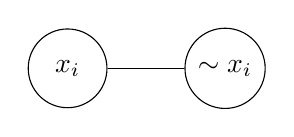
\begin{tikzpicture}[state/.style={circle, draw, minimum size=1cm}]
				      \node[state] (xi) {\( x_i \)};
				      \node[state, right of=xi, xshift=1cm] (nxi) {\( \sim x_i \)};

				      \draw[-] (xi) edge (nxi);
			      \end{tikzpicture}
		      \end{figure}

		      \newpage

		      Then for each clause \( \{l_{j,1}, l_{j,2}, l_{j,3}    \} \) , we construct a triangle, where exactly 2 vertices must be in the vertex cover.

		      \begin{figure}[ht]
			      \centering
			      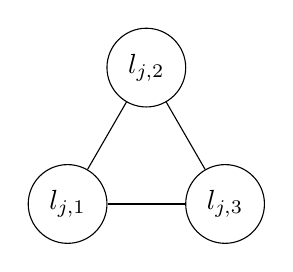
\begin{tikzpicture}[state/.style={circle, draw, minimum size=1cm}]
				      \node[state] (lj1) {\( l_{j,1} \)};
				      \node[state, xshift=2cm] (lj2) {\( l_{j,3} \)};
				      \node[state, xshift=1cm, yshift=1.732cm] (lj3) {\( l_{j,2} \)};

				      \draw[-] (lj1) edge (lj2);
				      \draw[-] (lj2) edge (lj3);
				      \draw[-] (lj3) edge (lj1);
			      \end{tikzpicture}
		      \end{figure}

		      For each clause, we connect each literal to the variable it represents, for example, given the clause \( x \lor \sim y \lor z \), it would look like

		      \begin{figure}[ht]
			      \centering
			      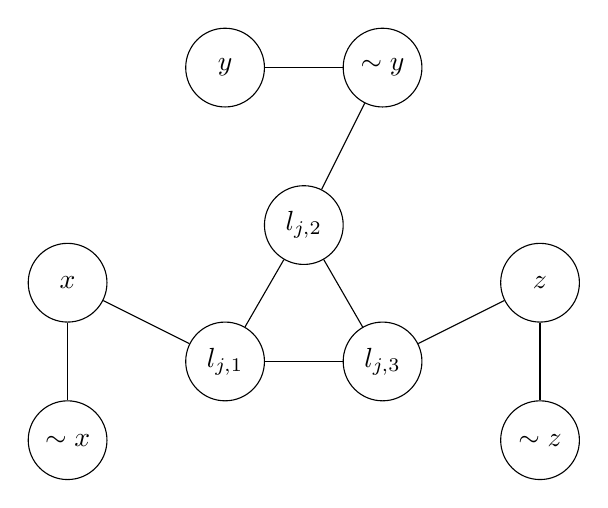
\begin{tikzpicture}[state/.style={circle, draw, minimum size=1cm}]
				      \node[state] (lj1) {\( l_{j,1} \)};
				      \node[state, xshift=1cm, yshift=1.732cm] (lj2) {\( l_{j,2} \)};
				      \node[state, xshift=2cm] (lj3) {\( l_{j,3} \)};

				      \node[state, left of=lj1, xshift=-1cm, yshift=1cm] (x) {\( x \)};
				      \node[state, left of=lj1, xshift=-1cm, yshift=-1cm] (nx) {\( \sim x \)};

				      \node[state, above of=lj2, xshift=-1cm, yshift=1cm] (y) {\( y \)};
				      \node[state, above of=lj2, xshift=1cm, yshift=1cm] (ny) {\( \sim y \)};

				      \node[state, right of=lj3, xshift=1cm, yshift=1cm] (z) {\( z \)};
				      \node[state, right of=lj3, xshift=1cm, yshift=-1cm] (nz) {\( \sim z \)};

				      \draw[-] (lj1) edge (lj2);
				      \draw[-] (lj2) edge (lj3);
				      \draw[-] (lj3) edge (lj1);

				      \draw[-] (x) edge (nx);
				      \draw[-] (lj1) edge (x);

				      \draw[-] (y) edge (ny);
				      \draw[-] (lj2) edge (ny);

				      \draw[-] (z) edge (nz);
				      \draw[-] (lj3) edge (z);
			      \end{tikzpicture}
		      \end{figure}

		      Now, selecting the right \( k \) allows us to choose exactly 2 literals in each clause and exactly 1 boolean assignment for each variables to be in the vertex cover,
		      we can use \( k = n + 2m \) for this.

		      The literal not choosen represents the literal we select to be true, since in each clause, only 1 of the literals need to be true for the whole clause to be true.
		      Since this literal was not choosen, then the variable that the literal is connected to must be choosen to be in the vertex cover.

		      Hence if there exists a vertex cover for this graph, there must be a satisfying truth assignment to each variable for the satisfiability problem.
		      And given a satisfiability problem and a correct assignment of truth values to each variable, we can simply select either \( x_i \) or \( \sim x_i \) to be in the cover,
		      and for each clause the variable is connected to, select the literals not connected to \( x_i \) or \( \sim x_i \).

		      Hence 3SAT \( \le _m^p \) Vertex Cover, and vertex cover is NP-complete.

	      \end{proof}

	\item Max cut

	      Given an undirected graph \( G = (V, E) \) and a positive integer \( K \le |E| \), is there a cut of \( G \) with size \( > K \)? A cut partitions the vertices into two sets \( (X, Y) \), the
	      size of the cut is the number of edges removed to form the partition.

	\item Independent set

	      Given a graph \( G = (V, E) \) and a positive integer \( K \le |V| \), is there a subgraph of size \( \ge K \) where no vertices are adjacent?

	      \begin{proof}

		      Given a graph \( G = (V,E) \), if \( V^{\prime}\subseteq V  \) is a vertex cover for \( G \), that means that \( V - V^{\prime}  \) is an independent set.
		      To see this, suppose \( \{u, v\} \subseteq V - V^{\prime}   \), then there cannot exist \( (u, v) \in E \) otherwise one of \( u \) or \( v \) will be in \( V^{\prime}  \).
		      Hence there exists no edges between any vertices in \( V^{\prime}  \).

		      In the other direction, if \( V^{\prime}  \) is an independent set for \( G \), then \( V - V^{\prime}  \) is a vertex cover.
	      \end{proof}

	\item Clique

	      Given a graph \( G = (V, E) \) and a positive integer \( K \le |V| \), is there a complete subgraph of size \( \ge K \)?
	      Basically finding a subgraph of \( G \) where every vertice is adjacent.

	      \begin{proof}
		      We can reduce independent set to clique problem. Given a graph \( G = (V,E) \), then there exists an independent set in \( G \) iff there exists a clique in \( \overline{G}  \).

		      This is trivial, if \( V^{\prime}  \) is an independent set, then no vertices are adjacent, so in the complement of the graph, all the vertices in \( V^{\prime}  \) will be adjacent to each other.
	      \end{proof}

	\item Hamiltonian circuit

	      Given a graph \( G = (V, E) \), does \( G \) contain a hamiltonian circuit? i.e is there a simple circuit that goes through all vertices exactly once?

	\item Partition

	      Given a finite set \( A \) and a size funtion where \( \forall a \in A, s(a) > 0 \), is there a subset \( A^{\prime}   \) of \( A \) such that \[
		      \sum_{a \in A^{\prime} } s(a) = \sum_{a \not \in A^{\prime}  } s(a)
		      .\]

	      \( s(a) \) is given in binary for every \( a \), so input length is proportional to \( |A| + \sum_{a \in A} \log s(a) \)

	\item Set cover

	      Given a finite set \( A \) and a number \( k \), a collection of subsets \( S = \{S_{1},S_{2},\ldots ,S_m\} \) whose union is \( A \),
	      is there a subset \( S^{\prime} \subseteq   S \) where \( |S^{\prime}| \le k  \) such that the union is still \( A \)?

	\item Traveling salesman problem

	      Given a complete weighted graph \( G = (V,E) \) and a bound \( B \), does there exist a hamiltonian circuit in \( G \) of weight \( \le B \)?

	      Weights and \( B \) are provided in binary, so length of input is proportional to \( |V| + |E| + \log B + \sum_{e \in E} \log w_e \)
\end{enumerate}

\subsection{Constant improvements}
Given that a language \( L \) can be accepted by some machine \( M \) that is \( S(n) \) space bounded,
then there exists a machine \( M^{\prime}  \) that can accept the same language with the same number of tapes in \( \left\lceil cS(n) \right\rceil  \) for some \( c > 0 \).

The idea is that each cell of \( M^{\prime}  \) represents \( m \) cells of \( M \), so if the tape alphabet of \( M \) is \( \Gamma \), then the tape alphabet for \( M^{\prime}  \) is \( \Gamma ^{m}  \),
so the space used by this machine is \( \left\lceil \frac{S(n)}{m} \right\rceil  \)

\hfill

The same idea can be applied to time complexity, given some conditions.
Our machine \( M \) must have \( k \ge 2 \) tapes, and must be \( T(n) \)  time bounded such that \( T(n) \not \in O(n) \), i.e. \( \lim_{n \to \infty} \frac{T(n)}{n} = \infty \).
Then we can construct \( M^{\prime}  \) that is \( \left\lceil cT(n) \right\rceil  \) time bounded for \( c>0 \)

The idea is to first apply the space compression so each cell takes up \( m \) cells of the original machine.
Then for every step of \( M^{\prime}  \), we look at the left and right neighbours of the current cell, this gives us \( 3m \) cells of information.
Since there is a finite number of states, this can be simulated by a DFA,
we can figure out whether the machine will accept, reject (including never halting), or move out of this \( 3m \) region.
This can be precomputed, so in the worst case our machine needs to take 8 steps (3 steps to read the region, 2 steps to write to the region, 3 steps to leave the region).

In one `basic' step, we have simulated at least m steps of \( M \),

\subsection{Some results}
\( DTIME(S(n)) \subseteq DSPACE(S(n)) \), i.e. you can not take more time than the amount of space you time, because using up 1 space requires 1 unit of time.

\hfill

If \( L \) is in \( DSPACE(S(n)) \), and \( S(n) \ge \log n \), then there exists a constant \( c \) depending on \( L \) such that L is in \( DTIME(c^{S(n)} ) \).
Intuitively since L is \( S(n) \) space bounded, there is a finite number of states the machine can be in, so you can take \( c \) to be \( |\Gamma|  \).

\hfill

If L is in \( NTIME(T(n)) \), then there exists a constant \( c \) depending on \( L \) such that  \( L \) is in \( DTIME(c^{T(n)} ) \).
Intuitively this is just a deterministic simulation of the non-deterministic TM.

\begin{theorem}
	Suppose \( S_{2}(n) \) and \( S_{1}(n) \) are both \( \ge \log n \) and \( S_{2}(n) \) is fully space constructible (uses exactly \( S(n) \) space on all inputs \( n \)) and
	\( S_{2}(n) \) grows faster than \( S_{1}(n) \), i.e. \( \lim_{n \to \infty} \frac{S_{1}(n)}{S_{2}(n)} = 0 \).
	Then there is a language in \( DSPACE(S_{2}(n)) - DSPACE(S_{1}(n)) \).
\end{theorem}

\begin{proof}
	Construct \( M \) that is \( S_{2}(n) \) space bounded, has a fixed number of tapes (at least 3), and let \( L \) denote the language accepted by \( M \).
	We show that \( L \) will not be in \( DSPACE(S_{1}(n)) \).

	\hfill

	\( M \) rejects all inputs of the form \( 1^{k}  \).

	\( M \) on input of the form \( 1^{k}0x  \):

	\tab Mark out space \( S_{2}(|1^{k}0x| ) \) on the work tape.
	This is needed to figure out how much space \( S_{2}(|1^{k}0x| ) \) takes, and allows us to reject when the simulation crosses this boundary.

	\tab Simulate \( M_x \) on the same input, if the simulation attempts to use more than \( S_{2}(|1^{k}0x |) \) space, then reject.

	\tab Else if \( M_x \) halts on the same input, then \( M \) accepts iff \( M_x \) did not accept the input.

	In the above simulation, we assume that \( M_x \) uses only 2 tapes and uses the alphabet \( \{0, 1, B\} \). Note that \( M \) is also \( S_{2}(n) \) space bounded, hence \( L \) is in \( DSPACE(S_{2}(n)) \).

	\hfill

	Suppose by way of contradiction that \( M^{\prime}  \) is a \( S_{1}(n) \) space bounded machine that accepts \( L \).
	Then we can construct a 2 tape machine \( M_x \) that accepts \( L \) and is also \( S_{1}(n) \) space bounded. WLOG we can assume \( M_x \) halts on all inputs.

	Now we try to simulate \( M_x \) on \( M \), let \( k \) be large enough such that \( c S_{1}(|1^{k}0x| ) < S_{2}(|1^{k}0x| ) \),
	then we know that this simulation must complete, and \( M \) either accepts or rejects.
	Then \( M \) accepts \( 1^{k}0x  \) iff \( M_x  \) did not, this is a contradiction as \( 1^{k}0x  \) should be accepted by both machines.

	Thus there can not be a machine \( M^{\prime}  \) that accepts \( L \) and is \( S_{1} \) space bounded.

\end{proof}


\begin{theorem}
	Suppose \( T_{2}(n) \) is fully time constructible and \( T_{2}(n), T_{1}(n) \ge  (1+\epsilon )n \). Suppose that \( T_{2}(n) \) grows faster than \( T_{1}(n) \)
	by more than a log factor, i.e. \( \lim_{n \to \infty} \frac{T_{1}(n) \log (T_{1}n)}{T_{2}(n)} = 0 \)
	(because turing machine simulation is \( n \log  n \)).

	Then there exists a language in \( DTIME(T_{2}(n)) \) but not in \( DTIME(T_{1}(n)) \)
\end{theorem}

The proof is very similar to space hierarchy, we just have the nlogn restriction from the universal turing machine.

\begin{proof}
	Construct \( M \) that is \( O(T_{2}(n)) \) time bounded, has a fixed number of tapes (at least 5), and let \( L \) denote the language accepted by \( M \).
	We show that \( L \) will not be in \( DTIME(T_{1}(n)) \).

	\hfill

	\( M \) rejects all inputs of the form \( 1^{k}  \).

	\( M \) on input of the form \( 1^{k}0x  \):

	\tab Mark out \( T_{2}(|1^{k}0x| ) \) on the work tape, so that we can count how many steps is taken.
	This allows us to reject when the simulation uses more time than \( T_{2}(|1^{k}0x| ) \)

	\tab Simulate \( M_x \) on the same input, if the simulation attempts to use more than \( T_{2}(|1^{k}0x |) \) time, then reject.

	\tab Else if \( M_x \) halts on the same input, then \( M \) accepts iff \( M_x \) did not accept the input.

	In the above simulation, we assume that \( M_x \) uses only 2 tapes and uses the alphabet \( \{0, 1, B\} \).
	Note that \( M \) is \( O(T_{2}(n)) \) space bounded, hence \( L \) is in \( DTIME(T_{2}(n)) \) by linear speedup theorem.

	\hfill

	Suppose by way of contradiction that \( M^{\prime}  \) is a \( T_{1}(n) \) time bounded machine that accepts \( L \).
	Then we can construct a 2 tape machine \( M_x \) that simulates \( M \) and accepts \( L \) and is \( cT_{1}(n)\log T_{1}(n) \) time bounded. WLOG we can assume \( M_x \) halts on all inputs.

	Now we try to run \( M_x \) on \( M \), let \( k \) be large enough such that \( c T_{1}(|1^{k}0x| ) \log T_{1}(|1^{k}0x| ) < T_{2}(|1^{k}0x| ) \),
	then we know that this simulation must complete, and \( M \) either accepts or rejects.
	Then \( M \) accepts \( 1^{k}0x  \) iff \( M_x  \) did not, this is a contradiction as \( 1^{k}0x  \) should be accepted by both machines.

	Thus there can not be a machine \( M^{\prime}  \) that accepts \( L \) and is \( T_{1} \) time bounded.

\end{proof}


\end{document}
